\documentclass[a4paper, 12pt]{article}
\usepackage[utf8x]{inputenc}
\usepackage{cmap}
\usepackage[english, russian]{babel}
\usepackage{indentfirst}
\usepackage[left=20mm, top=20mm, right=20mm, bottom=20mm]{geometry}
\usepackage{tikz}
\usepackage{float}
\usepackage{amsmath, amsfonts, amssymb}
\usepackage{graphicx}
\usepackage{fancybox, fancyhdr}
\usepackage{hyperref}
\usepackage{listings}
\usepackage{caption}
\usepackage{subcaption}
\usepackage{xcolor}
\usepackage{paralist}
\usepackage{tabularx}
\pagestyle{fancy}
\fancyhf{}
\fancyhead[L]{Лабораторная работа №3}
\fancyhead[R]{Программирование промышленных роботов}
\fancyfoot[C]{\thepage}
\graphicspath{{images/}}
\usetikzlibrary{patterns}
\definecolor{LightGray}{gray}{0.95}
\definecolor{LightGray2}{gray}{0.7}
\lstdefinelanguage{MELFABASIC}{
    keywords={MVS, MVR, JOVRD,
              HOPEN, HCLOSE, DLY,
              MOV, END},
    sensitive=true,
    comment=[*],
    morecomment=[l]{;},
    morestring=[b]"
}
\lstdefinestyle{code}{
    language=MELFABASIC, % replace with needed language
    basicstyle=\footnotesize\ttfamily,
    backgroundcolor=\color{LightGray},
    showspaces=false,
    showstringspaces=false,
    showtabs=false,
    tabsize=4,
    captionpos=b,
    breaklines=true,
    breakatwhitespace=false,
    frame=single,
    rulecolor=\color{LightGray2},
    linewidth=\linewidth,
    keywordstyle=\color{blue}\bfseries,
    commentstyle=\color{green!40!black},
    stringstyle=\color{purple},
    escapeinside={\%*}{*)},
    inputencoding=utf8x,
    xleftmargin=0pt,
    framexleftmargin=0pt,
    framexrightmargin=0pt
}
\lstset{style=code}
\hypersetup{
    colorlinks=true,
    linkcolor=blue,
    filecolor=magenta,
    urlcolor=cyan,
    pdftitle={contents setup},
    pdfpagemode=FullScreen,
}
\setlength{\parskip}{1.5mm}
\setlength{\headheight}{15pt}
\setlength{\footskip}{15pt}
\allowdisplaybreaks
\DeclareMathOperator{\sinc}{sinc}
\newcommand{\frc}[2]{\raisebox{2pt}{$#1$}\big/\raisebox{-3pt}{$#2$}}

\begin{document}
    \begin{titlepage}

        \begin{center}
        
\includegraphics[width=0.3\textwidth]{itmo.png} % requires itmo.png in /images folder
        \vfill
        
        Федеральное государственное автономное образовательное учреждение высшего образования
        «Национальный Исследовательский Университет ИТМО»\\
        
        \vfill
        {\large\bf ЛАБОРАТОРНАЯ РАБОТА №3}\\
        {\large\bf «ПРОГРАММИРОВАНИЕ ПРОМЫШЛЕННЫХ РОБОТОВ»}\\
        {\large\bf «ФОРМИРОВАНИЕ КОМПЛЕКСНЫХ ТРАЕКТОРИЙ»}
        \vfill

        \begin{flushright}
            \begin{minipage}{.45\textwidth}
            {
                \hbox{Преподаватель:}
                \hbox{Громов В. С.}
                \hbox{}
                \hbox{Выполнили:}
                \hbox{Румянцев А. А., R3341}
                \hbox{Чебаненко Д. А., R3341}
                \hbox{Овчинников П. А., R3341}
                \hbox{Блохин С. О., R3342}
                \hbox{Тоскано О. Арасели Д. П., R3338}
                \hbox{}
                \hbox{Факультет: СУиР}
            }
            \end{minipage}
        \end{flushright}
        
        \vfill
                
        Санкт-Петербург\\
        2024
        \end{center}
    \end{titlepage}
    
    \tableofcontents

    \newpage
    \section{Цели выполнения работы}
    Захватить инструмент захватным устройством. Касаясь щупом
    инструмента, обойти весь контур изогнутой листовой детали (рисунок \ref{fig:stand}).
    При касании щупа детали загорятся светодиоды на инструменте,
    имитируя процесс сварки. По окончании обхода контура детали вернуть
    инструмент в исходное положение. При составлении программы
    использовать команды \texttt{MOV}, \texttt{MVS}, \texttt{MVR}, смещения по оси Z инструмента.
    \begin{figure}[H]
        \centering
        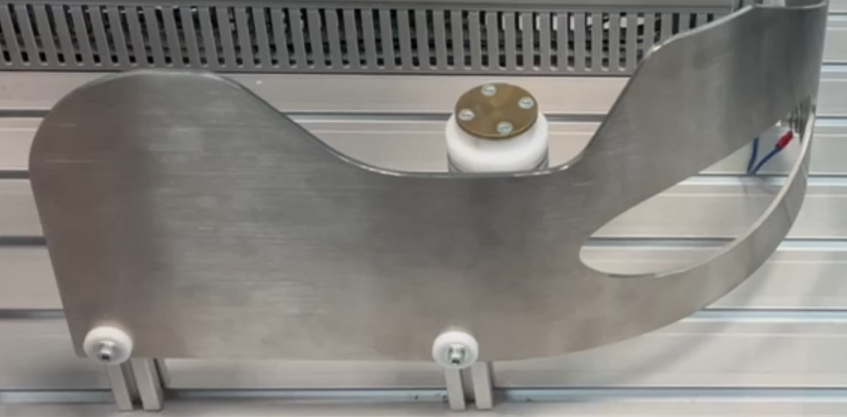
\includegraphics[scale=0.9]{stand.png}
        \captionsetup{skip=0pt}
        \caption{Листовая деталь для лабораторной работы}
        \label{fig:stand}
    \end{figure}


    \section{Код конечной программы}
    \begin{figure}[H]
        \centering
        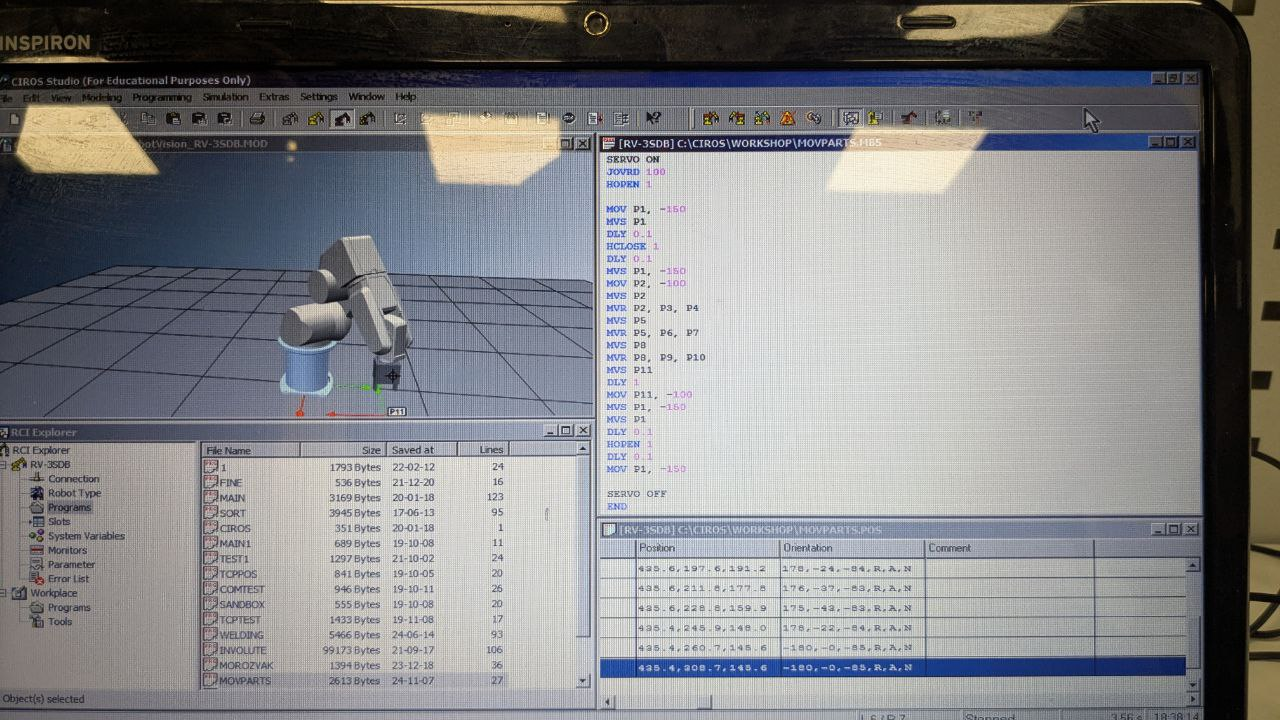
\includegraphics[scale=0.36]{code.jpg}
        \captionsetup{skip=0pt}
        \caption{Фото конечной программы}
        \label{fig:codephoto}
    \end{figure}
    \begin{lstlisting}[label=code, caption={Листинг конечной программы}]
    SERVO ON
    JOVRD 100
    HOPEN 1

    MOV P1, -150
    MVS P1
    DLY 0.1
    HCLOSE 1
    DLY 0.1
    MVS P1, -150
    MOV P2, -100
    MVS P2
    MVR P2, P3, P4
    MVS P5
    MVR P5, P6, P7
    MVS P8
    MVR P8, P9, P10
    MVS P11
    DLY 1
    MOV P11, -100
    MVS P1, -150
    MVS P1
    DLY 0.1
    HOPEN 1
    DLY 0.1
    MOV P1, -150

    SERVO OFF
    END
    \end{lstlisting}


    \subsection{Описание команд}
    При выполнении лабораторной работы использовались следующие команды программирования языка \texttt{MELFA BASIC}:
    \begin{compactitem}
    \item \texttt{END} -- завершение программы
    \item \texttt{SERVO ON} -- включение двигателей
    \item \texttt{JOVRD 100} -- скорость движения в процентах от максимальной
    \item \texttt{SERVO OFF} -- выключение двигателей
    \item \texttt{DLY 0.1} -- пауза выполнения программы в секундах
    \item \texttt{HOPEN 1} -- открытие захватного устройства
    \item \texttt{HCLOSE 1} -- закрытие захватного устройства 
    \item \texttt{MOV P1, -150} -- движение в точку P1 из таблицы сохраненных точек со смещением 150 мм вверх по оси Z
    \item \texttt{MVS P1} -- точное движение в точку P1 по прямой линии
    \item \texttt{MVR P2, P3, P4} -- движение по дуге через точки P2, P3, P4 из таблицы сохраненных точек
    \end{compactitem}


    \section{Таблица сохраненных точек}
    \begin{figure}[H]
        \centering
        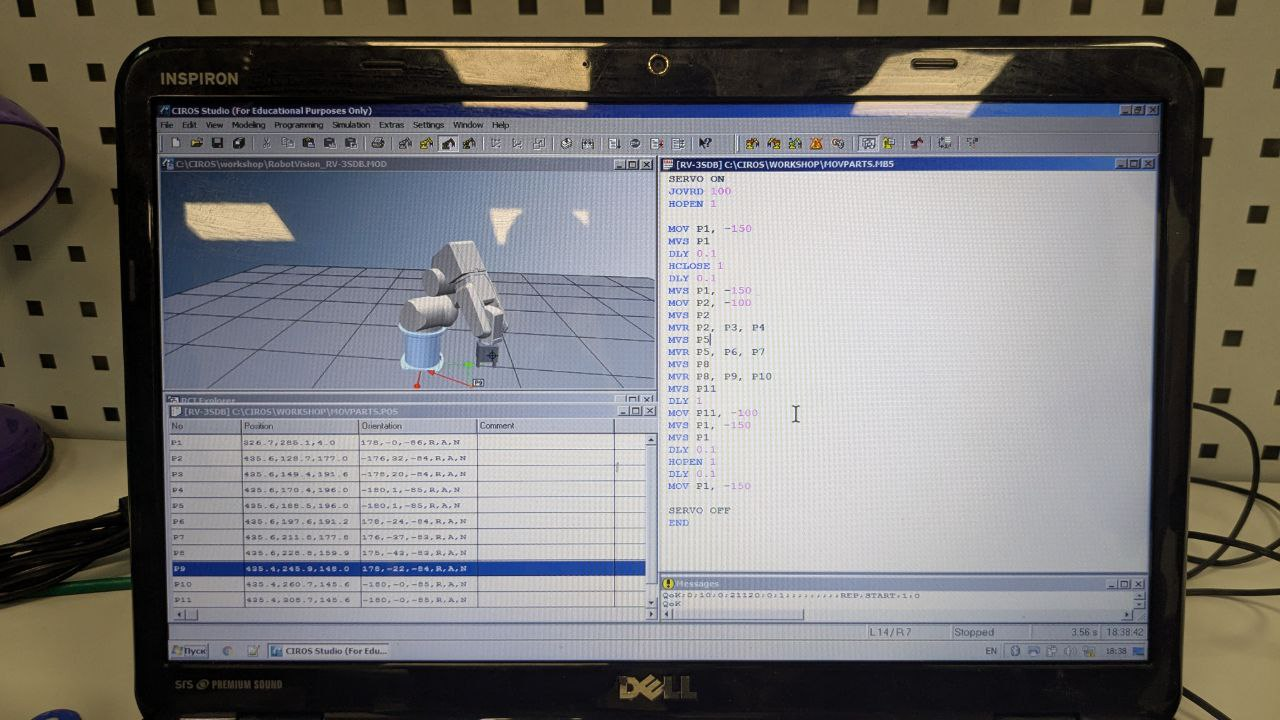
\includegraphics[scale=0.36]{table.jpg}
        \captionsetup{skip=0pt}
        \caption{Фото таблицы с сохраненными точками}
        \label{fig:table}
    \end{figure}
    \begin{tabularx}{0.92\textwidth} { 
        | >{\raggedright\arraybackslash}X 
        | >{\raggedright\arraybackslash}X 
        | >{\raggedright\arraybackslash}X | }
       \hline
       No & Position & Orientation \\
       \hline
       P1 & $326.7, 286.1, 4.0$ & $178, -0, -86$, R, A, N \\
       \hline
       P2 & $435.6, 128.7, 177.0$ & $-176, 32, -84$, R, A, N \\
       \hline
       P3 & $435.6, 149.4, 191.6$ & $-178, 20, -84$, R, A, N \\
       \hline
       P4 & $435.6, 170.4, 196.0$ & $-180, 1, -85$, R, A, N \\
       \hline
       P5 & $435.6, 188.5, 196.0$ & $-180, 1, -85$, R, A, N \\
       \hline
       P6 & $435.6, 197.6, 191.2$ & $178, -24, -84$, R, A, N \\
       \hline
       P7 & $435.6, 211.0, 177.0$ & $176, -37, -82$, R, A, N \\
       \hline
       P8 & $435.6, 228.8, 159.9$ & $175, -42, -82$, R, A, N \\
       \hline
       P9 & $435.4, 245.9, 148.0$ & $178, -22, -84$, R, A, N \\
       \hline
       P10 & $435.4, 260.7, 145.6$ & $-180, -0, -85$, R, A, N \\
       \hline
       P11 & $435.4, 208.7, 145.6$ & $-180, -0, -85$, R, A, N \\
      \hline
    \end{tabularx}


    \section{Этапы выполнения программы}
    \begin{figure}[H]
        \centering
        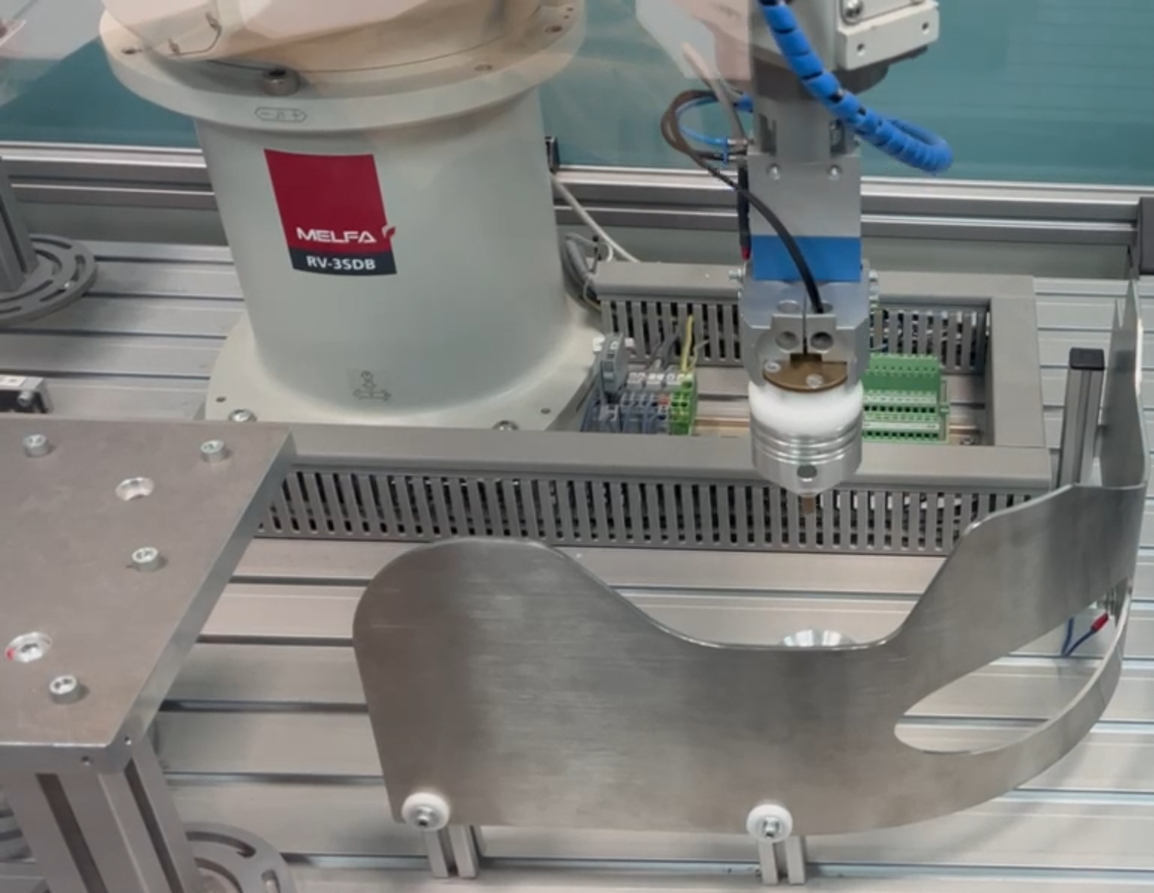
\includegraphics[scale=0.55]{take.png}
        \captionsetup{skip=0pt}
        \caption{Робот взял инструмент и поднялся}
        \label{fig:take}
    \end{figure}
    \begin{figure}[H]
        \centering
        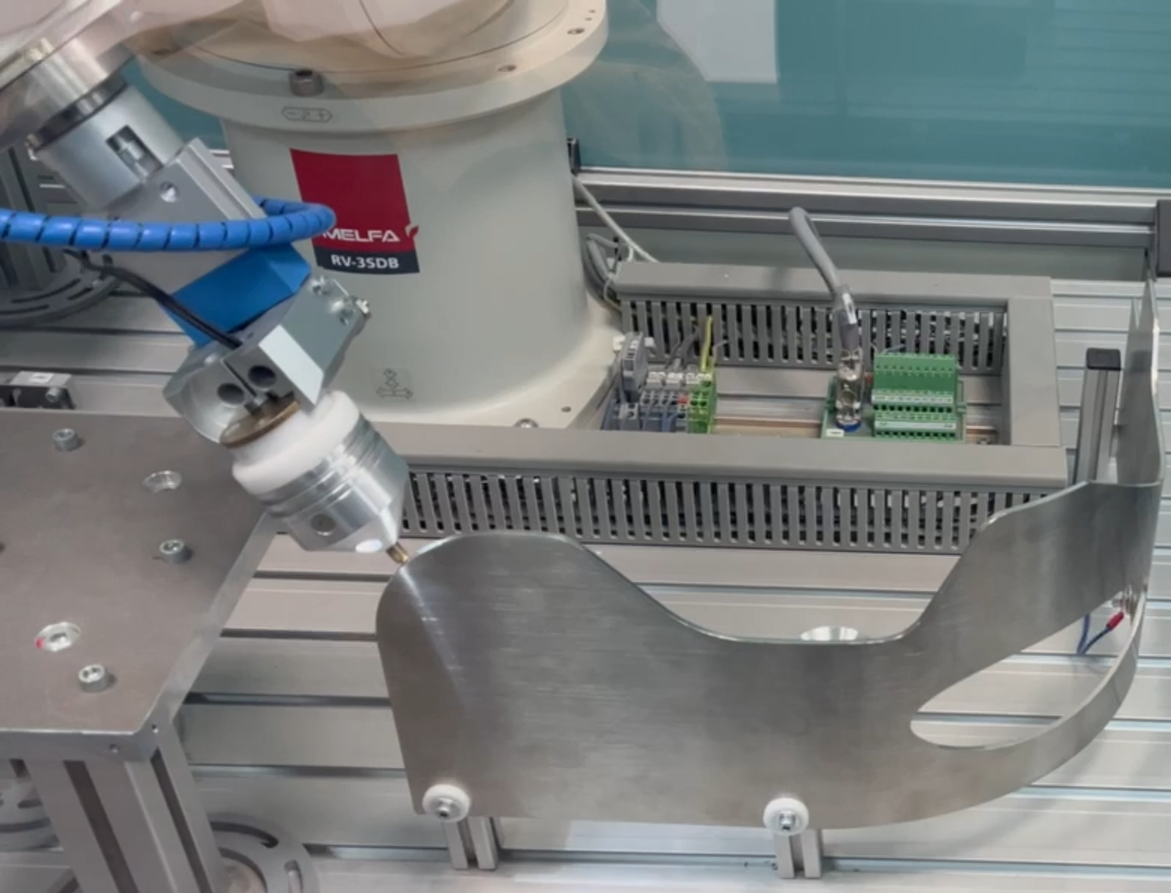
\includegraphics[scale=0.55]{scr1.png}
        \captionsetup{skip=0pt}
        \caption{Робот пришел к первой точке на кривой, опустился и начал процесс <<сварки>>}
        \label{fig:start}
    \end{figure}
    \begin{figure}[H]
        \centering
        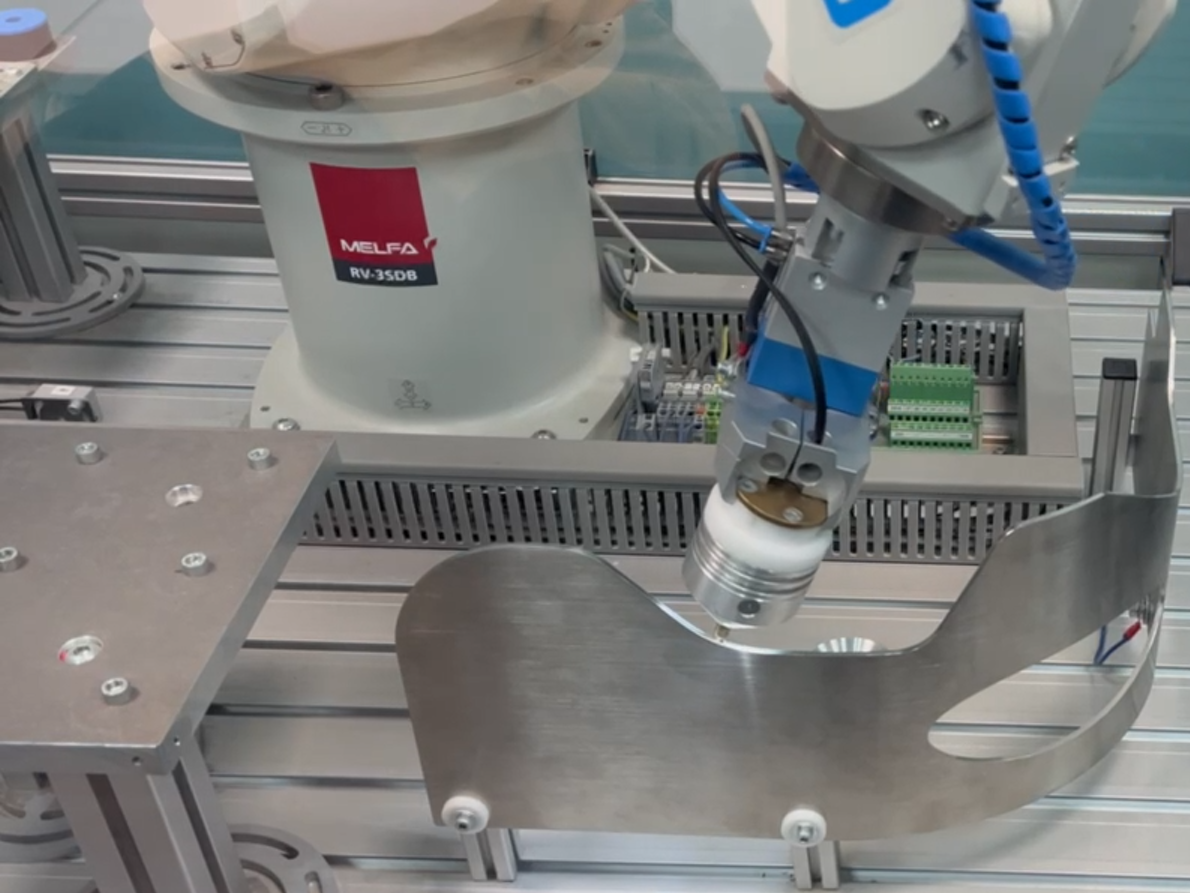
\includegraphics[scale=0.55]{scr3.png}
        \captionsetup{skip=0pt}
        \caption{Робот проходит траекторию и доходит до конца}
        \label{fig:scr3}
    \end{figure}
    \begin{figure}[H]
        \centering
        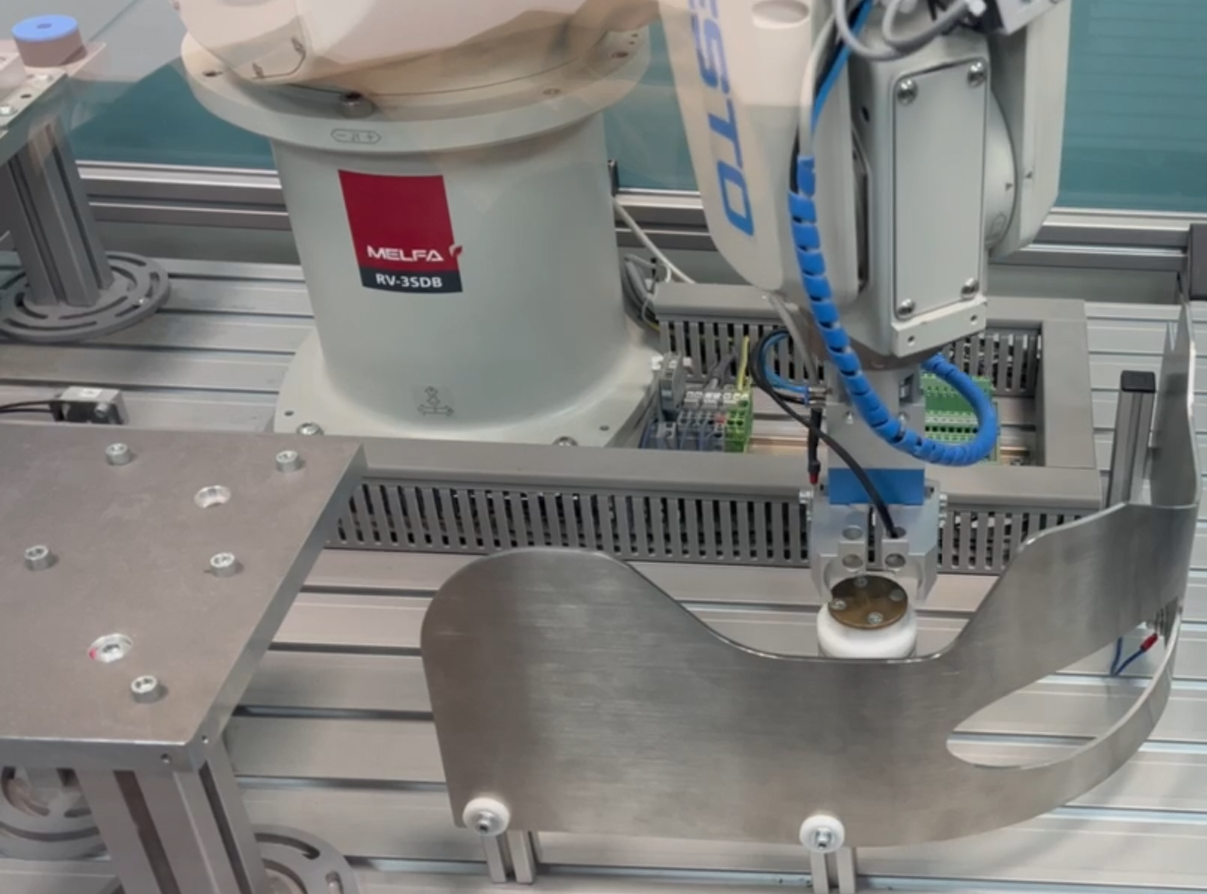
\includegraphics[scale=0.55]{end.png}
        \captionsetup{skip=0pt}
        \caption{Робот положил инструмент и начал подниматься на стартовую позицию}
        \label{fig:end}
    \end{figure}


    \newpage
    \section{Выводы}
    В результате выполнения лабораторной работы мы:
    \begin{compactitem}
        \item познакомились с точным движением \texttt{MVS} в точку и движением по дуге \texttt{MVR} через три точки
        \item написали программу на языке \texttt{MELFA BASIC} для прохождения роботом сложной траектории, используя различные способы движения к точкам и по ним
    \end{compactitem}
\end{document}